\documentclass[a4]{beamer}
\usepackage{amssymb}
\usepackage{graphicx}
\usepackage{subfigure}
\usepackage{newlfont}
\usepackage{amsmath,amsthm,amsfonts}
%\usepackage{beamerthemesplit}
\usepackage{pgf,pgfarrows,pgfnodes,pgfautomata,pgfheaps,pgfshade}
\usepackage{mathptmx}  % Font Family
\usepackage{helvet}   % Font Family
\usepackage{color}

\mode<presentation> {
 \usetheme{Default} % was
 \useinnertheme{rounded}
 \useoutertheme{infolines}
 \usefonttheme{serif}
 %\usecolortheme{wolverine}
% \usecolortheme{rose}
\usefonttheme{structurebold}
}

\setbeamercovered{dynamic}

\title[MA4413]{Statistics for Computing \\ {\normalsize Lecture 1B}}
\author[Kevin O'Brien]{Kevin O'Brien \\ {\scriptsize Kevin.obrien@ul.ie}}
\date{Autumn Semester 2013}
\institute[Maths \& Stats]{Dept. of Mathematics \& Statistics, \\ University \textit{of} Limerick}

\renewcommand{\arraystretch}{1.5}

\begin{document}


\begin{frame}
\titlepage
\end{frame}

\frame{
(Brought over from last lecture)
\begin{enumerate}
\item Contingency Tables
\item Conditional Probability: Worked Examples
\item Joint Probability Tables
\item The Multiplication Rule
\item Law of Total Probability
\item Bayes' Theorem
\item Exam standard Probability Question#
\item Sampling (Samples and Populations)
\item Sampling with and without Replacement
\end{enumerate}

(Later in Class : A look at Descriptive Statistic)
}

%-------------------------------------------------------%
\frame{
\frametitle{Multiplication Rule}
The multiplication rule is a result used to determine the probability that two events, $A$ and $B$, both occur.
The multiplication rule follows from the definition of conditional probability.\\ \bigskip

The result is often written as follows, using set notation:
\[ P(A|B)\times P(B) = P(B|A)\times P(A) \qquad \left( = P(A \cap B) \right) \]

Recall that for independent events, that is events which have no influence on one another, the rule simplifies to:
\[P(A \cap B)  = P(A)\times P(B) \]
}
%-------------------------------------------------------%
\frame{
\frametitle{Multiplication Rule}
From the first year intake example, check that
\[ P(E|F)\times P(F) = P(F|E)\times P(E)\]
\begin{itemize}
\item $P(E|F)\times P(F) = 0.58 \times 0.38  = 0.22$
\item $P(F|E)\times P(E) = 0.55 \times 0.40  = 0.22$
\end{itemize}
}
%------------------------------------------------------------%
\frame{
\frametitle{Law of Total Probability}
The law of total probability is a fundamental rule relating marginal probabilities to conditional probabilities. The result is often written as follows, using set notation:
\[ P(A)  = P(A \cap B) + P(A \cap B^c) \]

where $P(A \cap B^c)$ is probability that event $A$ occurs and $B$ does not.\\ \bigskip


Using the multiplication rule, this can be expressed as
\[ P(A) = P(A | B)\times P(B) + P(A | B^{c})\times P(B^{c}) \]
}
%------------------------------------------------------------%
\frame{
\frametitle{Law of Total Probability}
From the first year intake example , check that
\[ P(E)  = P(E \cap M) + P(E \cap F) \]
with $ P(E) = 0.40$, $ P(E \cap M) = 0.18$ and  $ P(E \cap F) = 0.22$
\[ 0.40  = 0.18 + 0.22 \]
\textbf{Remark:}  $M$ and $F$ are complement events.

}

%------------------------------------------------------------%
\frame{
\frametitle{Bayes' Theorem}
Bayes' Theorem is a result that allows new information to be used to update the conditional probability of an event.
\bigskip

Recall the definition of conditional probability:
\[ P(A|B) = \frac{P(A \cap B)}{P(B)} \]


Using the multiplication rule, gives Bayes' Theorem in its simplest form:

\[ P(A|B) = \frac{P(B|A)\times P(A)}{P(B)} \]

}

%------------------------------------------------------------%

\frame{
\frametitle{Probability: Worked Example }
An electronics assembly subcontractor receives resistors from two suppliers: Deltatech provides
70\% of the subcontractors's resistors while another company, Echelon, supplies the remainder.
\\
1\% of the resistors provided by Deltatech fail the quality control test, while 2\% of the
resistors from Echelon also fail the quality control test.

\begin{enumerate}
\item What is the probability that a resistor will fail the quality control test?
\item What is the probability that a resistor that fails the quality control test was supplied by Echelon?
\end{enumerate}
}

%------------------------------------------------------------%

\frame{
\frametitle{Probability: Worked Example}
Firstly, let's assign names to each event.
\begin{itemize}
\item $D$ : a randomly chosen resistor comes from Deltatech.
\item $E$ : a randomly chosen resistor comes from Echelon.
\item $F$ : a randomly chosen resistor fails the quality control test.
\item $P$ : a randomly chosen resistor passes the quality control test.
\end{itemize}
\bigskip
We are given (or can deduce) the following probabilities:
\begin{itemize}
\item $P(D) = 0.70$,
\item $P(E) = 0.30$.
\end{itemize}

}
%------------------------------------------------------------%

\frame{
\frametitle{Probability: Worked Example}

We are given two more important pieces of information:
\begin{itemize}
\item The probability that a randomly chosen resistor fails the quality control test, given that it comes from Deltatech: $P(F|D) = 0.01 $.
\item The probability that a randomly chosen resistor fails the quality control test, given that it comes from Echelon: $P(F|E) = 0.02$.
\end{itemize}

}
%------------------------------------------------------------%

\frame{
\frametitle{Probability: Worked Example}

The first question asks us to compute the probability that a randomly chosen resistor fails the quality control test. i.e. $P(F)$.\\
\bigskip
All resistors come from either Deltatech or Echelon. So, using the \textbf{\emph{law of total probability}}, we can express $P(F)$ as follows:

\[ P(F)  = P(F \cap D) + P(F \cap E) \]

}

%------------------------------------------------------------%

\frame{
\frametitle{Probability: Worked Example}

Using the \textbf{\emph{multiplication rule}}  i.e. $P(A \cap B) = P(A|B) \times P(B)$, we can re-express the formula as follows

\[ P(F)  = P(F|D) \times P(D) + P(F|E) \times P(E) \]

We have all the necessary probabilities to solve this.

\[ P(F)  = 0.01 \times 0.70 + 0.02 \times 0.30   = 0.007 + 0.006  = 0.013\]

}

%------------------------------------------------------------%

\frame{
\frametitle{Probability: Worked Example}

\begin{itemize}
\item
The second question asks us to compute probability that a resistor that fails the quality control test was supplied by Echelon.
\item In other words; of the resistors that did fail the quality test only, what is the probability that a randomly selected resistor was supplied by Echelon?
\item We can express this mathematically as $P(E|F)$.
\item We can use \textbf{\emph{Bayes' theorem}} to compute the answer.
\end{itemize}


}
%------------------------------------------------------------%

\frame{
\frametitle{Probability: Worked Example}
Recall Bayes' theorem
\[ P(A|B) = \frac{P(B|A)\times P(A)}{P(B)} \]
\bigskip

\[ P(E|F) = \frac{P(F|E)\times P(E)}{P(F)}  =  \frac{0.02 \times 0.30}{0.013} = 0.46\]

}
\frame{
\frametitle{Sampling}
The major use of statistics is to use information from a \textit{\textbf{sample}} to infer something about a \textit{\textbf{population}}.
\begin{itemize}


\item A \textit{\textbf{population}} is a collection of data whose properties are analyzed. The population is the complete collection to be studied, it contains all subjects of interest.

\item A \textit{\textbf{sample}} is a part of the population of interest, a sub-collection selected from a population.

\item
A \textit{\textbf{parameter}} is a numerical measurement that describes a characteristic of a population, while a \textit{\textbf{sample statistic}} is a numerical measurement that describes a characteristic of a sample.

\item In general, we will use a statistic to infer something about a parameter. 
\end{itemize}
}


\frame{
\frametitle{Sampling without replacement}
\begin{itemize}
\item Sampling is said to be ``without replacement" when a unit is selected at random from the population and it is not returned to the main lot. \item The first unit is selected out of a population of size $N$ and the second unit is selected out of the remaining population of  $N-1$ units and so on.
    \item For example, if you draw one card out of a deck of 52, there are only 51 cards left to draw from if you are selecting a second card.
\end{itemize}
}

\frame{
\frametitle{Sampling without replacement}
A lot of 100 semiconductor chips contains 20 that are defective.
Two chips are selected at random, without replacement from the lot.
\begin{itemize}
\item What is the probability that the first one is defective? \\(Answer : 20/100 , i.e 0.20)
\item What is the probability that the second one is defective given that the first one was defective? \\(Answer: 19/99)
\item What is the probability that the second one is defective given that the first one was not defective? \\(Answer: 20/99)
\end{itemize}
}

\frame{
\frametitle{Sampling With Replacement }

Sampling is called ``with replacement" when a unit selected at random from the population is returned to the population and then a second element is selected at random. Whenever a unit is selected, the population contains all the same units.
\begin{itemize}
\item What is the probability of guessing a PIN number for an ATM card at the first attempt.

\item Importantly a digit can be used twice, or more, in PIN codes.

\item For example $1337$ is a valid pin number, where $3$ appears twice.

\item
We have a one-in-ten chance of picking the first digit correctly, a one-in-ten chance of the guessing the second, and so on.

\item All of these events are independent, so the probability of guess the correct PIN is $0.1 \times 0.1 \times 0.1 \times 0.1 = 0.0001$
\end{itemize}
}
%--------------------------------------------------------%
\frame{
\frametitle{Descriptive Statistics}

We will digress from Probabilility for a while, and look at \textbf{Descriptive Statistics}.
\begin{itemize}
%\item Sampling without replacement.
%\item Factorials
%\item Permutations
%\item Combinations
%\item Relative Frequency and Frequency tables
%\item Histograms
\item Sample Mean
\item Sample Median
\item Measures of dispersion
%\item Expected Values
\end{itemize}

}





%--------------------------------------------------------%

\section{Descriptive Statistics}

\frame{

\frametitle{Descriptive Statistics}

\begin{itemize}
\item Measures of Centrality
\begin{itemize}
\item Mean
\item Median
\end{itemize}
\item Measures of Dispersion
\begin{itemize}
\item Range
\item Variance
\item Standard Deviation
\end{itemize}
% \item Quantiles
% \item Distribution of data ( Skewed or Symmetric )
\end{itemize}

}
%--------------------------------------------------------%
\frame{
\frametitle{Measures of Centrality}

\begin{itemize}
\item Measures of centrality give one representative number for the location of the centre of the distribution of data.
\item
The most common measures are the \textbf{\emph{mean}} and the \textbf{\emph{ median }}.
\item We must make a distinction between a sample mean and a population mean: The sample mean is simply the average of all the items in a sample.  \item The population mean (often represented by the Greek letter $\mu$) is simply the average of all the items in a population. \item Because a population is usually very large, the population mean is usually an unknown constant.
\item We will return to the matter of population means in due course. For now, we will look at sample means.
\end{itemize}

}
%----------------------------------------------------------------%
\frame{
\frametitle{Sample Mean}

\begin{itemize}
\item The sample mean is an estimator available for estimating the population mean . It is a measure of location, commonly called the average, often denoted $\bar{x}$, where $x$ is the data set.
\item
Its value depends equally on all of the data which may include outliers. It may not appear representative of the central region for skewed data sets.
\item
It is especially useful as being representative of the whole sample for use in subsequent calculations.
\item The sample mean of a data set is defined as :
\[ \bar{x} = { \sum x_i\over n}\]
\item $\sum x_i$ is the summation of al the elements of $x$, and $n$ is the sample size.
\end{itemize}
}
%----------------------------------------------------------------%
\frame{
\frametitle{Computing the sample mean}

Suppose we roll a die 8 times and get the following scores: $x = \{ 5, 2, 1, 6, 3, 5, 3, 1\}$ \\ \bigskip

What is the sample mean of the scores $\bar{x}$?
\[ \bar{x}  = {5 + 2 +  1 +  6 +  3 +  5 +  3 +  1 \over 8 } = {26 \over 8} =  3.25 \]



}

%--------------------------------------------------------%
\begin{frame}[fragile]
\frametitle{Using \texttt{R} to compute mean (and median)}
When implementing this in R, we would use the following code

\begin{verbatim}
> # create the "vector" x with the required values
> x=c(5, 2, 1, 6, 3, 5, 3, 1)
>
> mean(x)
[1] 3.25
>
> # See next slides first.
> sort(x)
[1] 1 1 2 3 3 5 5 6
> median(x)
[1] 3
\end{verbatim}

\end{frame}
%----------------------------------------------------------------%
\frame{
\frametitle{Median}
\begin{itemize}
\item The other commonly used measure of centrality is the median.

\item The median is the value halfway through the ordered data set, below and above which there lies an equal number of data values.
\item For an odd sized data set, the median is the middle element of the \textbf{ordered} data set.
\item For an even sized data set, the median is the average of the middle pair of elements of an \textbf{ordered} data set.
\item It is generally a good descriptive measure of the location which works well for \textbf{\emph{skewed data}}, or data with \textbf{\emph{outliers}}.

\item For later, the median is the 0.5 quantile, and the second quartile $Q_2$.
\end{itemize}
}

%----------------------------------------------------------------%
\frame{
\frametitle{Computing the median}
\textbf{Example:}


With an odd number of data values, for example nine, we have:
\begin{itemize}
\item Data : $\{96, 48, 27, 72, 39, 70, 7, 68, 99 \}$
\item Ordered Data :  $\{7, 27, 39, 48, 68, 70, 72, 96, 99\}$
\item Median : 68, leaving four values below and four values above
\end{itemize}
\bigskip
With an even number of data values, for example 8, we have:
\begin{itemize}
\item Data : $\{96, 48 ,27 ,72, 39, 70, 7, 68  \}$
\item Ordered Data : $\{7, 27, 39, 48, 68, 70, 72, 96\}$
\item Median : Halfway between the two 'middle' data points - in this case halfway between 48 and 68, and so the median is 58
\end{itemize}
}

%--------------------------------------------------------%
\begin{frame}[fragile]
\frametitle{Using \texttt{R} to compute mean (and median)}
When implementing this in \texttt{R}, we would use the following code

\begin{verbatim}
> x1=c(96, 48, 27, 72, 39, 70, 7, 68, 99 )
> sort(x1)
[1]  7 27 39 48 68 70 72 96 99
> median(x1)
[1] 68
>
> x2=c(96, 48 ,27 ,72, 39, 70, 7, 68)
> sort(x2)
[1]  7 27 39 48 68 70 72 96
> median(x2)
[1] 58
\end{verbatim}

\end{frame}
%--------------------------------------------------------%
\frame{
\frametitle{Dispersion }

\begin{itemize}
\item The data values in a sample are not all the same. This variation between values is called \textbf{ \emph{dispersion}}.

\item When the dispersion is large, the values are widely scattered; when it is small they are tightly clustered.

%The width of diagrams such as dot plots, box plots, stem and leaf plots is greater for samples with more dispersion and vice versa.

\item
There are several measures of dispersion, the most common being the variance and  standard deviation. These measures indicate to what degree the individual observations of a data set are dispersed or 'spread out' around their mean.

\item
In engineering and science, high precision is associated with low dispersion.
\end{itemize}
}




%--------------------------------------------------------%
\frame{
\frametitle{Range}

\begin{itemize}
\item The range of a sample (or a data set) is a measure of the spread or the dispersion of the observations. \item It is the difference between the largest and the smallest observed value of some quantitative characteristic and is very easy to calculate.

\item A great deal of information is ignored when computing the range since only the largest and the smallest data values are considered; the remaining data are ignored.

\item The range value of a data set is greatly influenced by the presence of just one unusually large or small value in the sample (outlier).
\end{itemize}

\textbf{Example}


The range of $\{65,73,89,56,73,52,47\}$ is $ 89-47 = 42$.

% If the highest score in a 1st year statistics exam was 98 and the lowest 48, then the range would be 98-48 = 50.

}


%--------------------------------------------------------%


\frame{
\frametitle{Introducing Variance}

Consider the three data sets $X$, $Y$ and $Z$
\begin{itemize}
\item $X= \{900,925,950,975,1025,1050,1075,1100 \}$
\item $Y=\{900,905,910,920,1080,1090,1095,1100\}$
\item $Z=\{900,985,990,995,1005,1010,1015,1100\}$
\end{itemize}

For each of the data sets, the following statements can be verified

\begin{itemize}
\item The mean of each data set is 1000
\item There are 8 elements in each data set
\item The minima and maxima are 900 and 1100 for each set
\item The range is 200.
\end{itemize}

From the plot on the next slide, notice how different the three data sets are in terms of dispersion around the mean value.

}

%--------------------------------------------------------%

\frame{
\frametitle{Introducing Variance}


\begin{center}
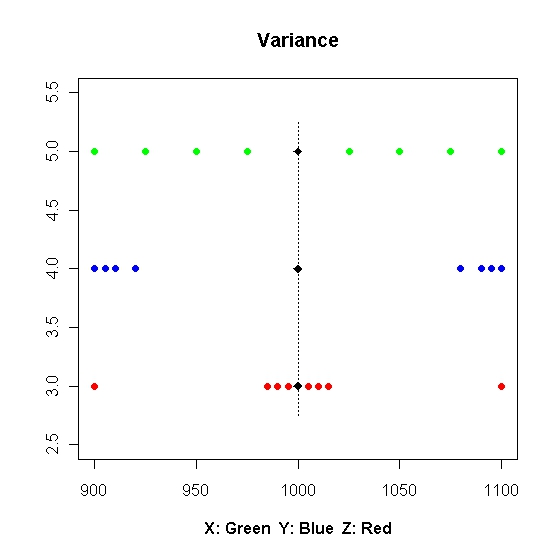
\includegraphics[scale=0.4]{2AVariance}
\end{center}

}

%--------------------------------------------------------%
\frame{
\frametitle{Variance}


\begin{itemize}

\item The (population) variance of a random variable is a non-negative number which gives an idea of how widely spread the values are likely to be; the larger the variance, the more scattered the observations on average.

\item Stating the variance gives an impression of how closely concentrated round the expected value the distribution is; it is a measure of the 'spread' of a distribution about its average value.

\item We distinguish between population variance (denoted $\sigma^2$) and sample variance (denoted $s^2$). For now, we will look only at sample variance.

\end{itemize}

}


%-------------------------------------------------------------------------%
\frame{

\frametitle{Sample Variance}

\begin{itemize}

\item Sample variance is a measure of the spread of or dispersion within a set of sample data.

\item The sample variance is the sum of the squared deviations from their mean divided by one less than the number of observations in the data set.

\item For example, for $n$ observations $x_1, x_2, x_3, \ldots , x_n$  with sample mean $\bar{x}$, the sample variance is given by


 \[ s^2 = { \sum (x-\bar{x})^2  \over n-1}\]




\end{itemize}
}
%--------------------------------------------------%
\frame{
\frametitle{Sample Standard Deviation}
\begin{itemize}
\item Standard deviation is the square root of variance
\item Standard deviation is commonly used in preference to variance because it is denominated in the same units as the mean.
\item For example, if dealing with time units, we could have a variance of something like $25$ \emph{ square minutes }, whereas the equivalent standard deviation is 5 minutes.
\item Population standard deviation is denoted  $\sigma$.
\item Sample standard deviation is denoted $s$.
\end{itemize}
}

%--------------------------------------------------------%
\begin{frame}[fragile]
\frametitle{Using \texttt{R}}Using \texttt{R} to compute standard deviation and variance for these data sets.

\begin{verbatim}
> X=c(900,925,950,975,1025,1050,1075,1100)
> Y=c(900,905,910,920,1080,1090,1095,1100)
> Z=c(900,985,990,995,1005,1010,1015,1100)
>
> sd(X);sd(Y);sd(Z)
[1] 73.19251
[1] 97.87018
[1] 54.37962
> 
>var(X);var(Y);var(Z)
[1] 5357.143
[1] 9578.571
[1] 2957.143
\end{verbatim}
\end{frame}

\end{document}

%--------------------------------------------------------%
\section{ Combinations and Permutations }

%--------------------------------------------------------%
\frame{
\frametitle{Factorials Numbers}

A factorial is a positive whole number, based on a number $n$ , and which is written as $``n!"$. The factorial $n!$ is defined as follows:

\[n!  =n \times (n-1) \times (n-2) \times \ldots \times 2 \times 1 \]

Remark $n!  =n \times (n-1)!$\\ \bigskip

\textbf{ Example: }

\begin{itemize}
\item $3!  = 3 \times 2  \times 1 = 6 $

\item $4!  = 4 \times 3! = 4 \times 3 \times 2 \times 1 = 24$
\end{itemize}
Remark $0! = 1$ not $0$.


}

%--------------------------------------------------------%
\frame{
\frametitle{Permutations and Combinations}


Often we are concerned with computing the number of ways of selecting and arranging groups of items. \begin{itemize} \item  A \textbf{\emph{combination}} describes the selection of items from a larger group of items.  \item A \textbf{\emph{permutation}} is a combination that is arranged in a particular way.
\end{itemize}

\bigskip
\begin{itemize}
\item Suppose we have items A,B,C and D to choose two items from.
\item AB is one possible selection, BD is another. AB and BD are both combinations.
\item More importantly, AB is one combination, for which there are two distinct permutations: AB and BA.
\end{itemize}
}

%--------------------------------------------------------%
\frame{
\frametitle{Combinations}

\textbf{Combinations: }
The number of ways of selecting $k$ objects from $n$ unique objects is:

\[ ^n C_k = {n!  \over k! \times (n-k)!} \]

In some texts, the notation for finding the number of possible combination is written

\[ ^n C_k =  {n \choose k} \]

}

%--------------------------------------------------------%
\frame{
\frametitle{Example of Combinations}
How many ways are there of selecting two items from possible 5?

\[ ^5 C_2   \left( \mbox{ also }  {5 \choose 2}  \right) =  {5!  \over 2! \times 3!} =  {5 \times 4 \times 3!  \over 2 \times 1 \times 3!} = 10  \]

\bigskip
Discuss how combinations can be used to compute the number of rugby matches for each group in the Rugby World Cup.

}
%--------------------------------------------------------%
\frame{
\frametitle{The Permutation Formula}
The number of different permutations of r items from n unique items is written as $^n P_k$


\[ ^n P_k = \frac{n!}{(n-k)!}\]
}

%--------------------------------------------------------%
\frame{
\frametitle{Permutations}
\textbf{Example:}
How many ways are there of arranging 3 different jobs, between 5 workers, where each worker can only do one job?


\[ ^5 P_3 = \frac{5!}{(5-3)!}  = {5! \over 2!} = 60\]

}



%--------------------------------------------------------%
\frame{
\frametitle{Example of Combinations}

A committee of 4 must be chosen from 3 females and 4 males.

\begin{itemize}
\item In how many ways can the committee be chosen.
\item In how many cans 2 males and 2 females be chosen.
\item Compute the probability of a committee of 2 males and 2 females are chosen.
\item Compute the probability of at least two females.
\end{itemize}
}

%--------------------------------------------------------%
\frame{
\frametitle{Example of Combinations}

\textbf{Part 1}

We need to choose 4 people from 7:

This can be done in

\[
^7 C_4  = {7!  \over 4! \times 3!} =  {7 \times 6 \times 5 \times 4!  \over 4! \times 3!} = 35 \mbox{ ways.}
\]


\textbf{Part 2}

With 4 men to choose from, 2 men can be selected in \[
^4 C_2  = {4!  \over 2! \times 2!} =  {4 \times 3 \times 2!  \over 2! \times 2!} = 6\mbox{ ways.}
\]

Similarly 2 women can be selected from 3 in
\[
^3 C_2  = {3!  \over 2! \times1!} =  {3 \times 2!  \over 2! \times 1!} = 3\mbox{ ways.}
\]

}

%--------------------------------------------------------%
\begin{frame}[fragile]
\frametitle{Using \texttt{R}}
When implementing combination calculations in \texttt{R}, we use the \texttt{choose()} function.

\begin{verbatim}
> choose(5,0)
[1] 1
> choose(5,1)
[1] 5
> choose(5,2)
[1] 10
> choose(5,3)
[1] 10
> choose(5,4)
[1] 5
> choose(5,5)
[1] 1
\end{verbatim}

\end{frame}
%--------------------------------------------------------%
\frame{
\frametitle{Example of Combinations}

\textbf{Part 2}

Thus a committee of 2 men and 2 women can be selected in $ 6 \times 3  = 18 $ ways.\\
\bigskip
\textbf{Part 3}

The probability of two men and two women on a committee is
\[ {\mbox{Number of ways of selecting 2 men and 2 women} \over \mbox{Number of ways of selecting 4 from 7}} = {18 \over 35 }\]

}
%--------------------------------------------------------%
\frame{
\frametitle{Example of Combinations}

\textbf{Part 4}
\begin{itemize}
\item The probability of at least two females is the probability of 2 females or 3 females being selected.
\item We can use the addition rule, noting that these are two mutually exclusive events.
\item From before we know that probability of 2 females being selected is 18/35.
\end{itemize}

}
%--------------------------------------------------------%
\frame{
\frametitle{Example of Combinations}

\textbf{Part 4}
\begin{itemize}
\item We have to compute the number of ways of selecting 1 male from 4 (4 ways) and the number of ways of selecting three females from 2 ( only 1 way)
\item The probability of selecting three females is therefore ${4 \times 1 \over 35} = 4/35$
\item So using the addition rule
\[ Pr(\mbox{ at least 2 females }) = Pr(\mbox{ 2 females }) + Pr(\mbox{ 3 females }) \]
\[ Pr(\mbox{ at least 2 females })  = 18/35 + 4/35 = 22/35 \]
\end{itemize}

}

\end{document}
%------------------------------------------------------------%
\frame{
\frametitle{Random Variables}
\begin{itemize} \item The outcome of an experiment need not be a number, for example, the outcome when a coin is tossed can be `heads' or `tails'. \item
However, we often want to represent outcomes as numbers. \item
A \textbf{\emph{random variable}} is a function that associates a unique numerical value with every outcome of an experiment.
\item The value of the random variable will vary from trial to trial as the experiment is repeated.
\item Numeric values can be assigned to outcomes that are not usually considered numeric. \item For example, we could assign a `head' a value of $0$, and a `tail' a value of $1$, or vice versa.
\end{itemize}
}
%------------------------------------------------------------%
\frame{
\frametitle{Random Variables}
There are two types of random variable - discrete and continuous. The distinction between both types will be important later on in the course.\\ \bigskip

\textbf{Examples}
\begin{itemize}
\item A coin is tossed ten times. The random variable X is the number of tails that are noted.
X can only take the values $\{0, 1, ..., 10\}$, so $X$ is a discrete random variable.
\item A light bulb is burned until it burns out. The random variable Y is its lifetime in hours.
Y can take any positive real value, so Y is a continuous random variable.
\end{itemize}
}

%--------------------------------------------------------------------------------%
\frame{
\frametitle{Discrete Random Variable}
\begin{itemize}
\item A discrete random variable is one which may take on only a countable number of distinct values such as $\{0, 1, 2, 3, 4, ... \}$.\item Discrete random variables are usually (but not necessarily) counts. \item If a random variable can take only a finite number of distinct values, then it must be discrete. \item Examples of discrete random variables include the number of children in a family, the Friday night attendance at a cinema, the number of patients in a doctor's surgery, the number of defective light bulbs in a box of ten.
    \end{itemize}
}


%--------------------------------------------------------------------------------%
\frame{
\frametitle{Continuous Random Variable}
\begin{itemize} \item
A continuous random variable is one which takes an infinite number of possible values. \item Continuous random variables are usually measurements. \item Examples include height, weight, the amount of sugar in an orange, the time required to run a computer simulation. \end{itemize}

}
\end{document}
%--------------------------------------------------------------------------------%
\frame{
\frametitle{The Monty Hall Problem}
\begin{itemize} \item Three cups. One contains the prize, the other two are empty
\item Choose one of the cups
\item What is the probability you have selected the right cup?
\end{itemize}

}
%--------------------------------------------------------------------------------%
\frame{
\frametitle{The Monty Hall Problem}
\begin{itemize} \item I am going to remove one of the empty cups, but not the one just selected.
\item There are two cups on the table, one with the prize, and one empty.
\item I offer you the choice to stick with your choice, or to switch you choice to the other remaining cup.
\item What is the best strategy here?
\end{itemize}
}
%--------------------------------------------------------------------------------%
\frame{
\frametitle{The Monty Hall Problem}
Strategies
\begin{itemize} \item It is better to stick with what you have chosen.
\item It is better to switch to the other cup.
\item It is doesn't matter.
\end{itemize}
}
%--------------------------------------------------------------------------------%
\frame{
\frametitle{The Monty Hall Problem}

The best strategy is to switch.
}

